\apendice{Documentación de usuario}
\label{sec:appendixE}

\section{Introducción}

En la sección anterior se ha descrito cómo instalar y configurar el entorno de desarrollo con Eclipse y KNIME SDK. Si solo se desea
utilizar la extensión desarrollada en un flujo de trabajo, sin ánimos de modificarla a nivel de código, podemos seguir las siguientes instrucciones
de instalación. 

\section{Instalación KNIME}

Como la extensión KNIME Moodle Integration se ha implementado en KNIME 4.7.7, instalaremos esta versión desde la sección \href{https://www.knime.com/download-previous-versions}{Previous Versions of KNIME}. 
KNIME está disponible para Windows, Linux y macOS.


\section{Instalación de la extensión Moodle KNIME Integration}

La extensión lista para ser utiliza en cualquier instalación de KNIME está disponible como pre-release en el repositorio del proyecto: 

\url{https://github.com/frankgil/knime-moodle/releases/tag/extension}

Para utilizar esta extensión, debemos ejecutar KNIME y crear un Sitio de actualización local 
(Local Update Site). Seguiremos estos pasos:
\

En primer lugar descargaremos y descomprimiremos en una carpeta local la extensión. 
\

Desde KNIME $\triangleright$ \english{Preferences} $\triangleright$ \english{Install/Update} $\triangleright$ \english{Available Software Sites} $\triangleright$ \english{Add}, añadiremos 
una ubicación local seleccionando la carpeta <<org.knime.moodle.update>>, tal y como se muestra en la Figura ~\ref{fig:usuario1}: 

\begin{figure}[!htb]
	\centering
	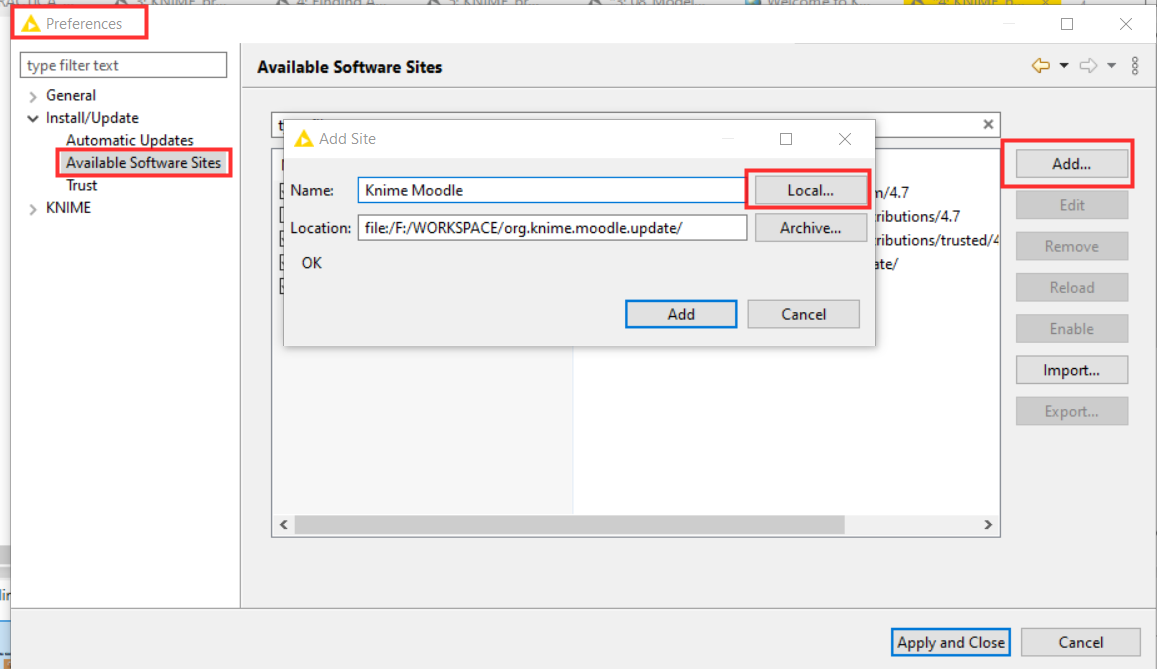
\includegraphics[width=1\textwidth]{img/manual_usuario_install_site_update1.png}
	\caption{Instalación de la extensión \node{Moodle} en KNIME 1.}
	\label{fig:usuario1}
\end{figure}
\FloatBarrier

A continuación seleccionamos el sitio añadido ~\ref{fig:usuario2},

\begin{figure}[!htb]
	\centering
	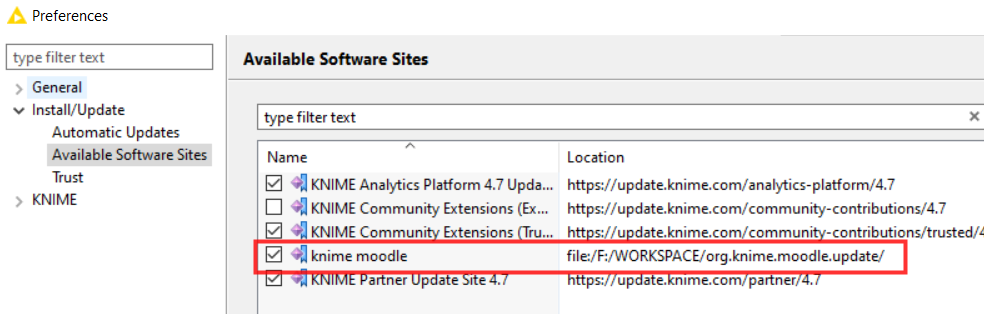
\includegraphics[width=1\textwidth]{img/manual_usuario_install_site_update2.png}
	\caption{Instalación de la extensión \node{Moodle} en KNIME 2.}
	\label{fig:usuario2}
\end{figure}
\FloatBarrier

y seleccionamos la instalación Moodle que queremos instalar ~\ref{fig:usuario3}.

\begin{figure}[!htb]
	\centering
	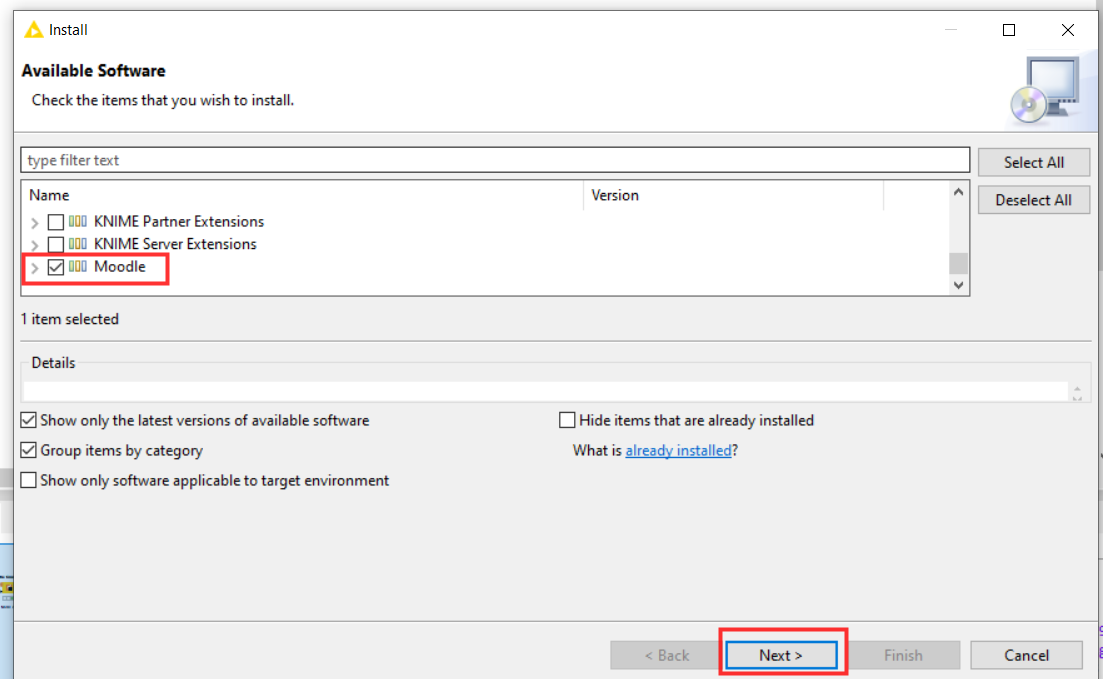
\includegraphics[width=1\textwidth]{img/manual_usuario_install_site_update3.png}
	\caption{Instalación de la extensión \node{Moodle} en KNIME 3.}
	\label{fig:usuario3}
\end{figure}
\FloatBarrier

Nos mostrará detalles de la extensión a instalar antes de completar la instalación ~\ref{fig:usuario4}. 

\begin{figure}[!htb]
	\centering
	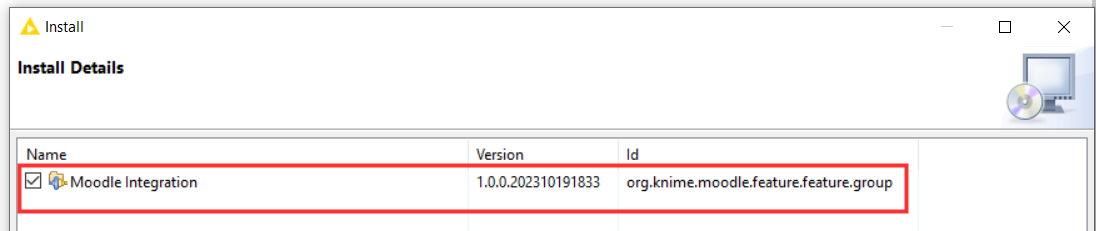
\includegraphics[width=1\textwidth]{img/manual_usuario_install_site_update4.png}
	\caption{Instalación de la extensión \node{Moodle} en KNIME 4.}
	\label{fig:usuario4}
\end{figure}
\FloatBarrier

Los nodos de la extensión \node{Moodle} se verán ahora en el repositorio de nodos ~\ref{fig:usuario5}. 

\begin{figure}[!htb]
	\centering
	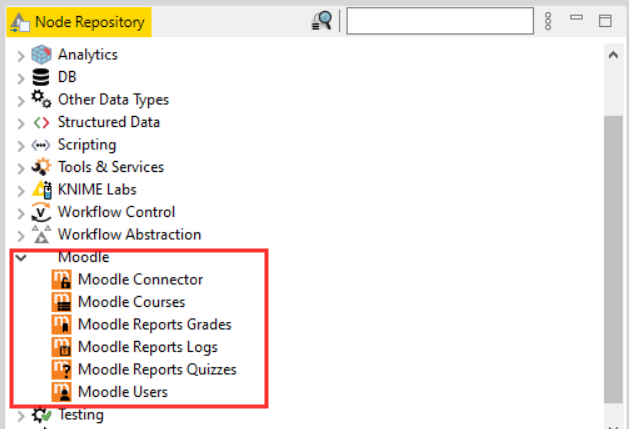
\includegraphics[width=1\textwidth]{img/manual_usuario_install_site_update5.png}
	\caption{Instalación de la extensión \node{Moodle} en KNIME 5.}
	\label{fig:usuario5}
\end{figure}
\FloatBarrier

\hphantom{ }

\newpage
\section{Crear un \english{workflow} y usar la extensión}

Ahora ya podremos crear \english{workflows} de KNIME incorporando los nodos de integración con Moodle y 
combinándolos con otros nodos de KNIME. Crea un nuevo Workflow desde \english{File} $\triangleright$ \english{New} $\triangleright$ \english{New KNIME Workflow} y sigue los siguientes pasos:  
\

Localiza en el repositorio de nodos el nodo \node{Moodle Connector} y añádelo al \english{Workflow} como se muestra en la Figura~\ref{fig:extension0}.

\begin{figure}[!htb]
	\centering
	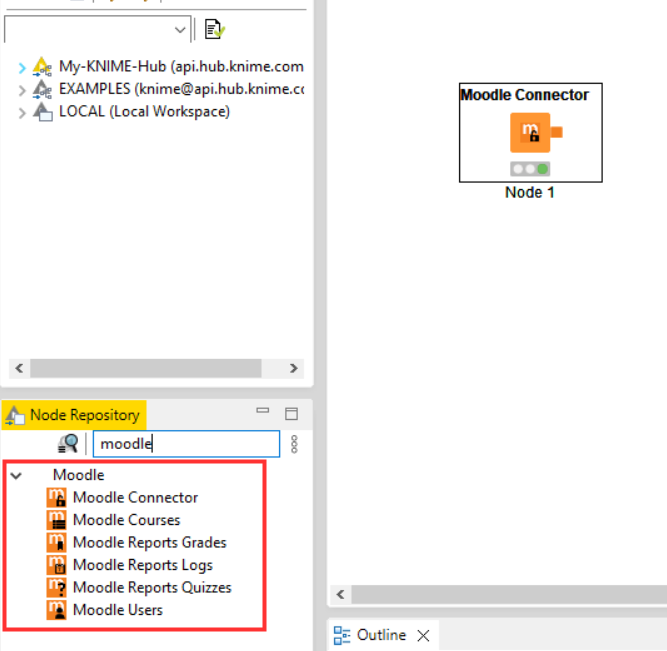
\includegraphics[width=1\textwidth]{img/manual_usuario_node_repository.png}
	\caption{Usando la extensión \node{Moodle}. Repositorio de nodos. }
	\label{fig:extension0}
\end{figure}
\FloatBarrier

Configura el nodo para conectar con una plataforma Moodle a la que tengas acceso ~\ref{fig:extension1}. 
\

\begin{figure}[!htb]
	\centering
	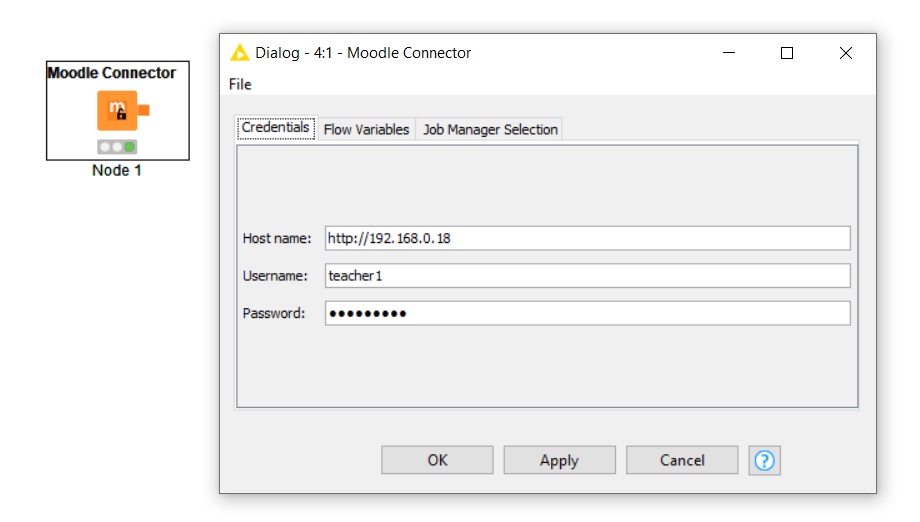
\includegraphics[width=1\textwidth]{img/manual_usuario_moodle_connector.png}
	\caption{Usando la extensión \node{Moodle} 1.}
	\label{fig:extension1}
\end{figure}
\FloatBarrier

Ejecuta el \english{workflow} y comprueba que se conecta correctamente a Moodle. En la información de 
depuración por Consola de KNIME~\ref{fig:extension2} verás las entradas \ruta{MoodleConnector} con 
información relativa al token de conexión, id del usuario y token del webservice. 
Si no recibes esta información, revisa que los datos de conexión en el nodo sean correctos. 
\

\begin{figure}[!htb]
	\centering
	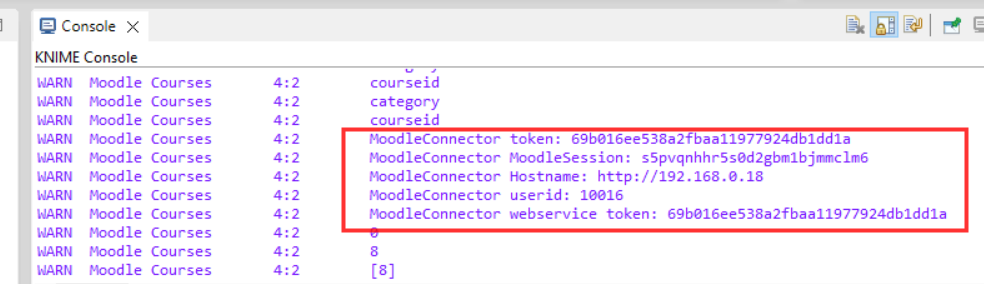
\includegraphics[width=1\textwidth]{img/manual_usuario_moodle_connector_login.png}
	\caption{Usando la extensión \node{Moodle} 2.}
	\label{fig:extension2}
\end{figure}
\FloatBarrier

Añade a continuación un nodo de tipo \node{Moodle Courses}. El nodo necesita como entrada la salida de un nodo de tipo \node{Table Creator}. 
Une los nodos y configura la tabla con dos columnas, \field{category} y \field{courseid} ~\ref{fig:extension3}. En estas columnas podrás indicar 
los identificados de categorías o cursos de tu plataforma Moodle. Aunque el contenido de la tabla 
es optativo, debe añadirse y enlazarse el nodo correspondiente. 

\begin{figure}[!htb]
	\centering
	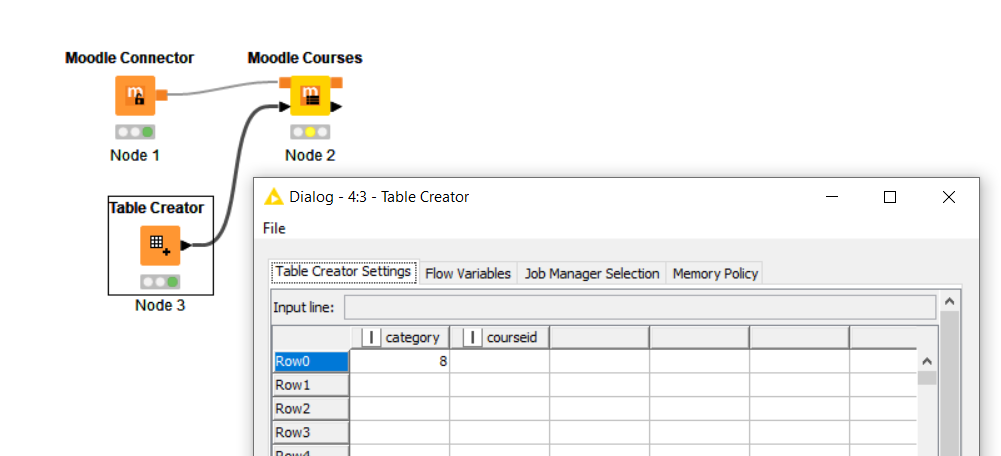
\includegraphics[width=1\textwidth]{img/manual_usuario_moodle_courses_table.png}
	\caption{Usando la extensión \node{Moodle} 3.}
	\label{fig:extension3}
\end{figure}
\FloatBarrier


En la configuración del nodo \node{Moodle Courses}, selecciona la columna 
correspondiente a la categoría y la correspondiente a los identificadores de cursos ~\ref{fig:extension4}. 

\begin{figure}[!htb]
	\centering
	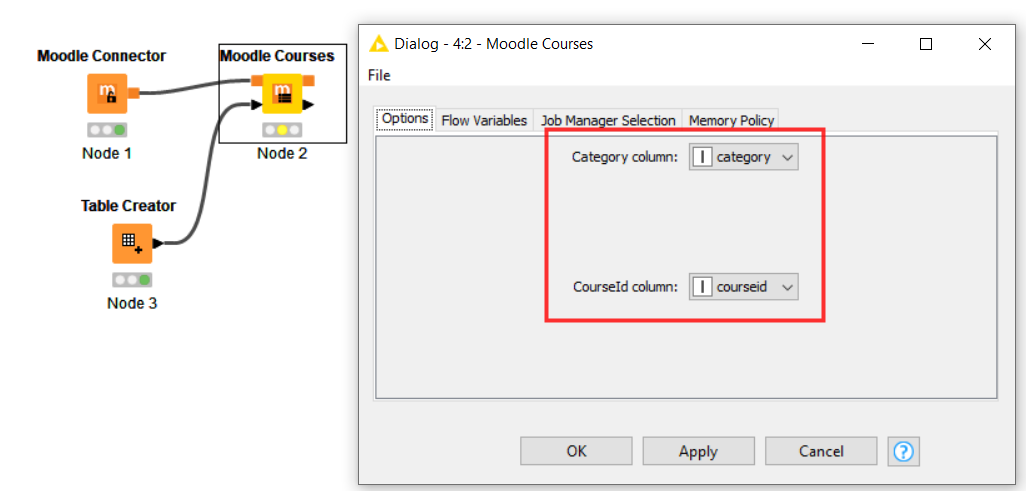
\includegraphics[width=1\textwidth]{img/manual_usuario_moodle_courses_config.png}
	\caption{Usando la extensión \node{Moodle} 4.}
	\label{fig:extension4}
\end{figure}
\FloatBarrier

Por último, ejecuta el \english{workflow} y comprueba la tabla de salida de \node{Moodle Courses}. Debes obtener una 
salida como la mostrada en la Figura ~\ref{fig:extension5}, con información de los cursos.  

\begin{figure}[!htb]
	\centering
	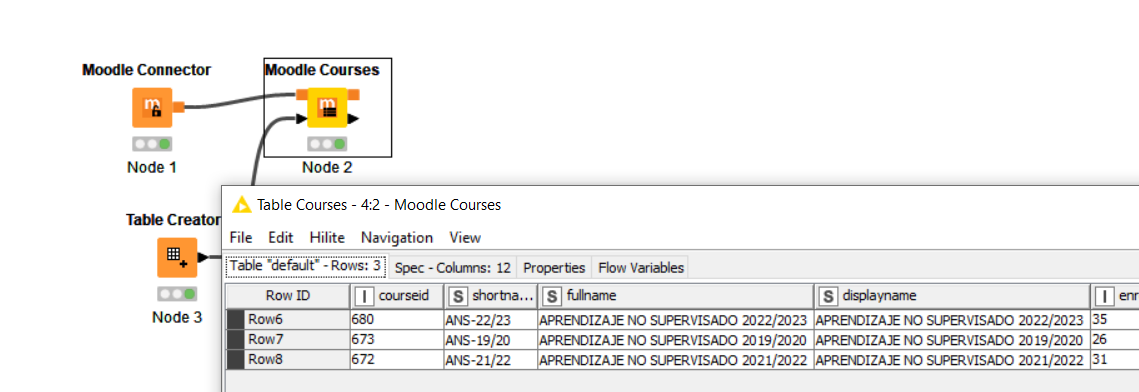
\includegraphics[width=1\textwidth]{img/manual_usuario_moodle_courses_list.png}
	\caption{Usando la extensión \node{Moodle} 5.}
	\label{fig:extension5}
\end{figure}
\FloatBarrier

A partir de aquí puedes añadir el resto de nodos de la extensión y combinarlos con otros nodos de KNIME. 
Consulta el Apéndice \ref{sec:appendixC} para saber más el diseño y funcionalidad de los nodos disponibles en la extensión \node{KNIME Moodle Integration}. 
